\documentclass{article}
\usepackage{amsmath,amsthm,amssymb}
\usepackage{mathtext}
\usepackage[T2A]{fontenc}
\usepackage[utf8]{inputenc}
\usepackage[english]{babel}
\usepackage{graphicx}
\usepackage{hyperref}
\usepackage{listings}


\title{Code Commenter}
\author{Edward Nee, Andrew Petropavlovskiy, Vladislav Annenkov}
\date{January 2023}



\begin{document}
\maketitle
\begin{abstract}
    This document describes our solution to the code2text problem. Here we have described the approaches to learn model and collect our own dataset. Here you can find our repository with notebook: \url{https://github.com/EdwardNee/CodeCommenter-NLP4Code}.
\end{abstract}



\section{Introduction}

The code is written for people and documentation comments are important part to make code more understandable. Popular libraries and frameworks contain documentation for public methods, but this doesn't apply to amateur code that makes up most of the open source code. The same can be said about commercial code because not all companies have a rule to write comments in their code.

So, the main idea behind this project is to solve this problem through docstring generation from source code and remove the task of writing comments from the developers.

\subsection{Team}

\begin{itemize}
  \item \textbf{Edward Nee} prepared this document;
  \item \textbf{Andrew Petropavlovskiy} prepared this document;
  \item \textbf{Vladislav Annenkov} prepared this document.
\end{itemize}



\section{Related Work}
\label{sec:related}

\subsection{LAMNER: Code Comment Generation Using Character Language Model and Named Entity Recognition}
In the paper \textit{LAMNER} \cite{lamnertoken} (Language Model and Named Entity Recognition) a Named Entity Recognition model is trained to learn the different types of code tokens. code tokens then fed into an encoder-decoder architecture to generate code comments.


\begin{figure}[!tbh]
    \centering
    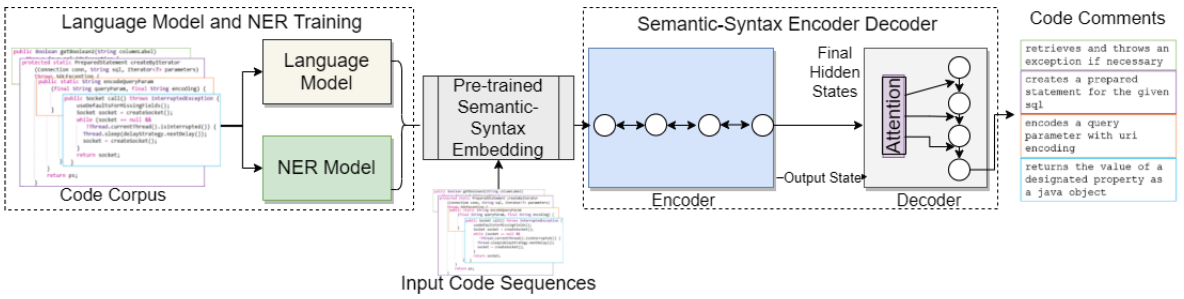
\includegraphics[width=1.0\linewidth]{lamner.png}
    \caption{Overview of LAMNER Framework}
    \label{fig:lamner}
\end{figure}

{Figure}~\ref{fig:lamner} illustrates the given framework of the LAMNER model. First left box depicts a bidirectional character-based language model and a NER model are trained separately on a code corpus that generates the input code embeddings for the next layer – Semantic-Syntax encoder decoder. Received raw embeddings are used as an input for the encoder. The decoder then uses the attention mechanism to decode the input code snippet into code comments.\\

\textit{Character-Level Language Model Architecture.} The authors showed architecture of the language model on figure~\ref{fig:bilstm}. It employs a single layer \textit{bidirectional LSTM}. The input to each LSTM unit is an embedding of a randomly initialized character. Each LSTM unit processes the embedding to generate the output and the next hidden state for the character. The output of the last unit is used to select the next output character with maximum likelihood. The model predicts the character l for the given sequence of \textit{public Boo}, which makes the last letter of \textit{public Bool} sequence.

\begin{figure}[h]
    \centering
    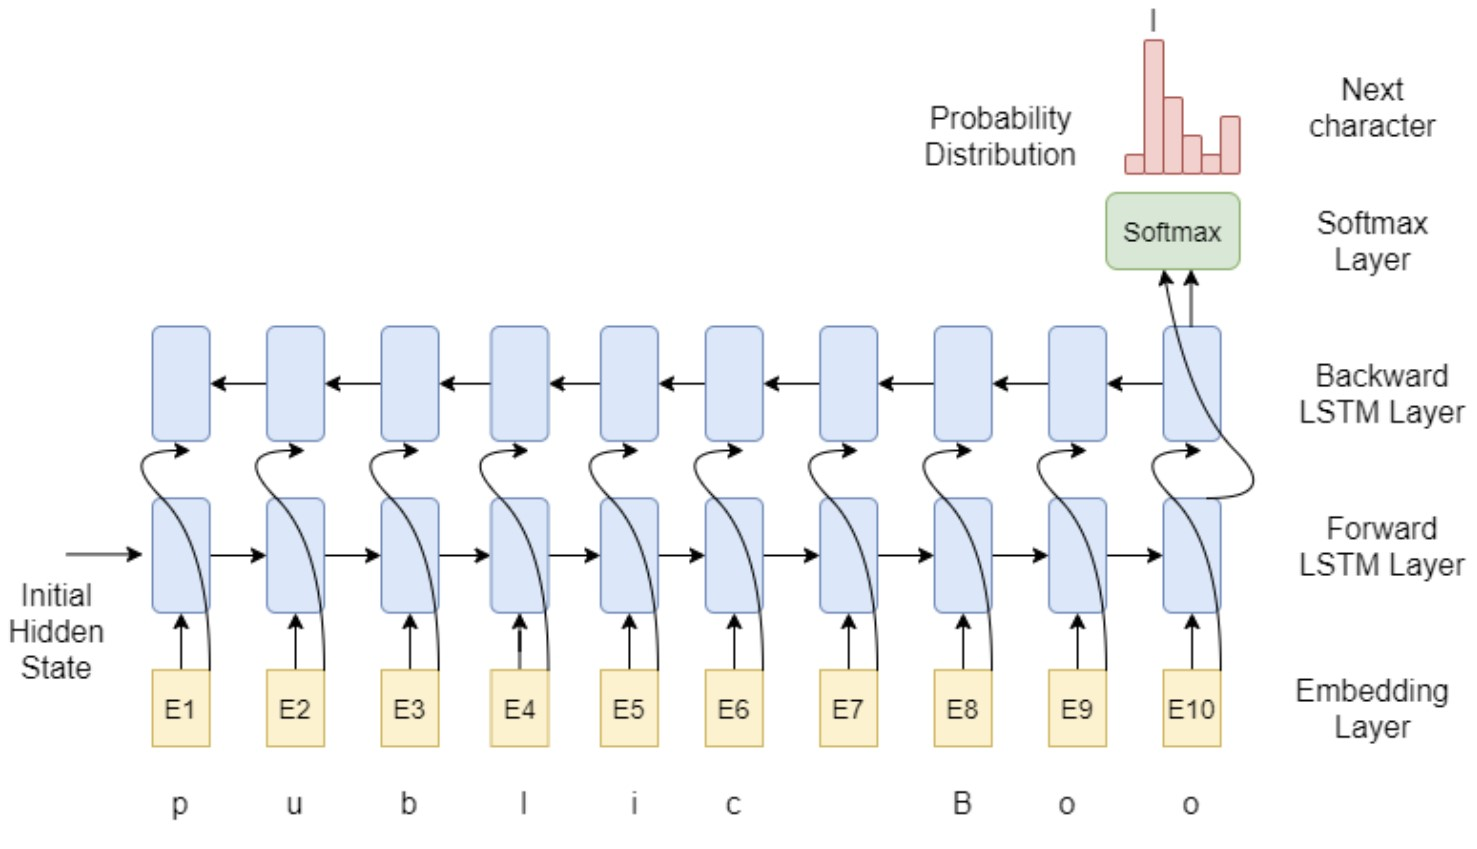
\includegraphics[width=1.0\linewidth]{bilstm.png}
    \caption{Overview of Character-Level Language Model Architecture.}
    \label{fig:bilstm}
\end{figure}

The article describes processing the code tokens with the code sequence, however, the \textit{AST} does not have a one-to-one mapping with code tokens, which is distinct in each programming language. NER is used to label the tokens of the code sequences. For example, the given code sequence \textit{public Boolean getBoolean2} ..., the token \textit{public} is labeled as \textit{modifier}, the token \textit{Boolean} is labeled as \textit{return type}, and the token \textit{getBoolean2} is labeled as \textit{function}.\\


The Semantic-Syntax encoder takes this semantic-syntactic embedding of the \textbf{code tokens} as input and models them together to output the semantic-syntax embeddings of the code sequence. Encoder processes the input using single layer bidirectional GRU. They use it due to its faster training time, and preservation the information for long sequences. \\ They say that the hidden state of the last token $h_{last}$ contains information of the complete sequence. This token then fed into a fully connected linear layer. The equation is: $y_{fc} = h_{last} * W_t + b$, where $W_t$ is weight matrix and $b$ is bias values matrix. \\
The final output is: $h_{final}=tanh(y_{fc})$ \\\\
The decoder with attention is trained in natural language. It implements Bahdanau’s mechanism on a unidirectional GRU. Model uses $h_{final}$ to
pay attention to the input sequence’s important tokens. The decoder will predict the next token until it reaches the maximum sequence length or the end of sentence token ⟨eos⟩.






\subsection{ComFormer: Code Comment Generation via Transformer and Fusion Method-based Hybrid Code Representation}
Authors introduced a new way of code commenting by combining transformers with hybrid code representation with AST information for better model learning.
They also evaluated the performance of ComFormer \cite{comformertoken} on a large Java code corpus with comments for that code.\\
First of all, authors got rid of OOV. They got tokens, which are the class names, variables and etc. Then they convert them into a sequences by dividing camel case names into a separated words. For example, getUserInfo() method will be converted to a sequence of get, user, info. After that, ComFormer uses BPE to convert each word of a sequence into a sequence of letters. The authors claim that with this mechanism, the generated comments will not contain words that are not in the data set.\\
Secondly, authors use AST representations in their model. They convert AST into a sequence for processing this data by the model. At start they used SBT method for that, but recently they created their own Sim\_SBT, which does not display unnecessary relationships, such as relationships with standard types and generates slightly shorter result, than SBT.
\begin{figure}[!tbh]
    \centering
    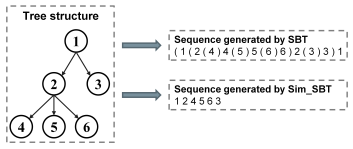
\includegraphics[width=1.0\linewidth]{sim-sbt.png}
    \caption{Sim\_SBT result}
    \label{fig:sim-sbt}
\end{figure}
ComFormer follows the Transformer architecture.\\
Encoder produces a sequence of context vectors $Z=(z_1,\dots,z_n)$. Input tokens are
passed through a standard embedding layer and then model uses another positional embedding layer. Than, encoded embeddings used as the input to the encoder of N layers. Every layer consists of multi-head attention mechanism and a feed-forward network. Attention calculated as $Attention(Q,K,V) = softmax(\frac{QK^{T}}{\sqrt{d_k}})$. Then the model calculates multi-headed attention and concatenate it with feed-forward layer.\\ $head_i = Attention(QW_{I}^Q, KW_{I}^K),VW_{I}^V$\\ $MultiHead(Q,K,V) = Concat_i(head_i)W^O$.\\\\
The second component of each layer is FFN:\\ $FFN(x) = max(0, xW_1 + b_1)W_2+b_2$\\
Authors use three different methods to fuse lexical and syntactical information of code end Encoder.\\\\
\textbf{Jointly Encoder} assumes that AST and code are two different inputs.\\
\textbf{Shared Encoder} encodes two inputs by weight sharing, switches two matrices together, adds linear layer and activates it.\\
\textbf{Single Encoder} splices inputs and and proceeds through word embeddings.

\begin{figure}[!tbh]
    \centering
    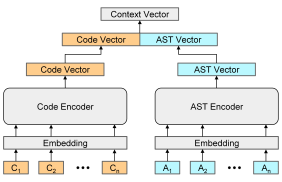
\includegraphics[width=0.6\linewidth]{jointly.png}
    \caption{Structure of Jointly fusion method in the Encoder}
    \label{fig:jointly}
\end{figure}
\begin{figure}[!tbh]
    \centering
    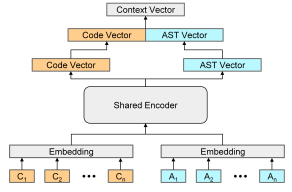
\includegraphics[width=0.6\linewidth]{shared.png}
    \caption{Structure of Shared fusion method in the Encoder}
    \label{fig:shared}
\end{figure}
\begin{figure}[!tbh]
    \centering
    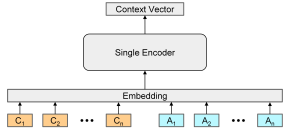
\includegraphics[width=0.6\linewidth]{single.png}
    \caption{Structure of Single fusion method in the Encoder}
    \label{fig:single}
\end{figure}
Then, model use standart Decoder to decode embeddings.\\
So, the whole model represented on figure 7.

\begin{figure}[!tbh]
    \centering
    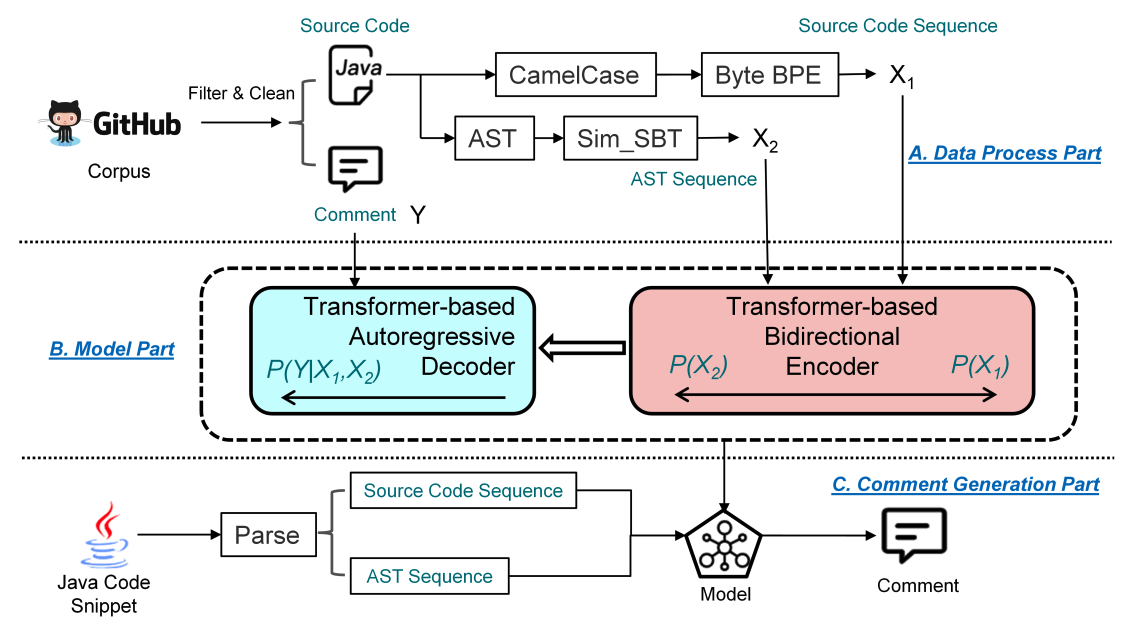
\includegraphics[width=1.0\linewidth]{comformer.png}
    \caption{Overview of ComFormer Framework}
    \label{fig:comformer}
\end{figure}

\section{Model Description}

To implement this task, we used the T5 model. T5 is an encoder-decoder model pre-trained on a multi-task mixture of unsupervised and supervised tasks and for which each task is converted into a text-to-text format. T5 works well on a variety of tasks out-of-the-box by prepending a different prefix to the input corresponding to each task.

We choose this model by two reasons:
\begin{itemize}
    \item This model achieves good results in different tasks.
    \item This model fits well for different tasks at the same time. So we don't need to implement difficult architecture for the our task.
\end{itemize}

Ideally, we would like to get a universal model to understand multiple programming languages and generate by that comment docs with various templates. By templates we mean some comment structure, because it can be different in some programming languages. For example, in C\# it is a XML-like doc comments while in Java it is simple text with a pinch of HTML tags.

To take this into account, we use two prefixes during training. In our task we've used Java and go programming languages:
\begin{itemize}
    \item "go docstring: ..." --- to translate code into go-like docstring;
    \item "java docstring: ..." --- to translate code into Java-like docstring.
\end{itemize}

Architecture of the resulting model and pipeline showed on {figure}~\ref{fig:model}.

\begin{figure}[!tbh]
    \centering
    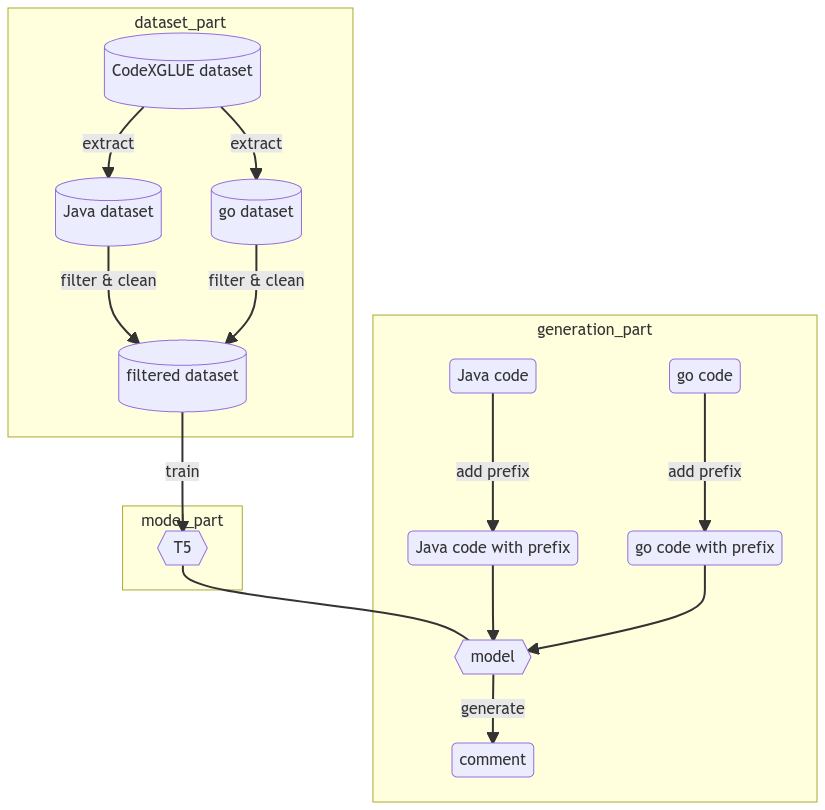
\includegraphics[width=1.0\linewidth]{model.png}
    \caption{Overview of our training-generation pipeline based on T5}
    \label{fig:model}
\end{figure}

\section{Dataset}

\subsection{Dataset Description}

For training the model, we used the CodeXGLUE dataset, which we have further refined for our task.

CodeXGLUE \cite{codexglue} stands for General Language Understanding Evaluation benchmark for CODE. It includes 14 datasets for 10 diversified programming language tasks covering code-code (clone detection, defect detection, cloze test, code completion, code refinement, and code-to-code translation), text-code (natural language code search, text-to-code generation), code-text (code summarization) and text-text (documentation translation) scenarios.

\subsection{Getting Dataset}

The dataset can be received in two ways: via GitHub and via HuggingFace. We've used HuggingFace that is popular solution for downloading pretrained models and datasets.

So, to download the dataset you can run the following method:
\begin{lstlisting}[language=Python]
import datasets
datasets.load_dataset(
    "code_x_glue_ct_code_to_text", # CodeXGLUE
    "java",                        # Programming language
    split="train")                 # train, valid, test
\end{lstlisting}

\subsection{Dataset Modifications and Markup}

To make dataset more usable we made some modifications for it.

First, we've added comment slashes in Java-part of the dataset. This makes it possible to use comments in our tools without any modification after generation. Just use our trained model as a full-fledged algorithm.

Second, we've combined datasets with different programming languages (Java and go) into unified dataset. To do this, we've added additional column with language name.

Statistics of our dataset showed in the {table}~\ref{tab:statistics}. The table shows data split between train, valid and test selections.

\begin{table}[tbh!]
\begin{center}
\begin{tabular}[t]{|l|ccc|}
\hline
%\cline{2-4}
 & Train & Valid & Test \\
\hline
Snippets & 332211 & 12508 & 19077 \\
Programming Languages & & 2 & \\
\hline
\end{tabular}
\caption{Statistics of our dataset}
\label{tab:statistics}
\end{center}
\end{table}

\section{Experiments}

\subsection{Metrics}

We use the cross entropy loss:

$$L = - \sum_{i=1}^n t_i \log{(p_i)},$$

for $n$ tokens, where $t_i$ is the truth label and $p_i$ is the Softmax probability for the $i^{th}$ token.

\subsection{Experiment Setup}

\subsubsection{Models}

We have tried two base models: \textit{BERT} and \textit{T5}. We stopped at T5 because this model provides better results for our task. Also T5 is used in articles with the same task as a model with the best training results.

\subsubsection{Datasets}

We have tried two datasets from CodeXGLUE: \textit{code2text} and \textit{text2code}. As a closer dataset to our task, code2text has gave better results during model training. Comparison of these datasets is shown in the {table}~\ref{tab:datasetscomparison}.

\begin{table}[tbh!]
\begin{center}
\begin{tabular}[t]{|l|cc|}
\hline
%\cline{2-3}
 & code2text & text2code \\
\hline
First epoch & 0.976 & 1.683 \\
Second epoch & 0.945 & 1.626 \\
Third epoch & ... & 1.618 \\
\hline
\end{tabular}
\caption{Dataset losses comparison}
\label{tab:datasetscomparison}
\end{center}
\end{table}

\subsection{Baselines}

...

\section{Results}

As a result, we got a model which translates programming code into docstring text. We haven't make special comparisons of our model with other models. Generation results showed in the {table}~\ref{tab:output1} and {table}~\ref{tab:output2}.

\begin{table}[!tbh]
    \centering
    \begin{tabular}{|l|}
\hline
java docstring: void printMessage(String message) \{ System.out.println(message); \}\\
\hline
// Prints a message.\\
//\\
// @param message the message to print.
\\
\hline
    \end{tabular}
    \caption{Java input and output sample}
    \label{tab:output1}
\end{table}

\begin{table}[!tbh]
    \centering
    \begin{tabular}{|l|}
\hline
go docstring: func CheckMdsAvailability() error \{ if conn, err :=\\net.Dial("unix", common.MetadataServiceRegSock); err != nil\\\{ return errUnreachable \} else \{ conn.Close() return nil \} \}\\
\hline
// CheckMdsAvailability checks whether a local metadata service can be reached.
\\
\hline
    \end{tabular}
    \caption{Go input and output sample}
    \label{tab:output2}
\end{table}

\section{Conclusion}

In our work we have received a complete solution for code2docstring task: adapted dataset, model setup and working pipeline.

To get an our own dataset we've worked on CodeXGLUE dataset, removed irrelevant data and concatenated datasets with different languages into one large dataset. Also we've added some programming language-specific decorations for docstring texts, like slashes in Java docstrings.

As a basic model, we have chosen the T5. T5 is a suitable solution to train multiple tasks in one model. We use it to implement different docstring types for various programming languages. Of course, we could use any other Transformer-based model to achieve this purpose, but we think, that pretrained T5 model with multitask-specific part has helped us achieve better results.

Finally, we have tested our model and got meaningful results. We think, that this solution can be improved later and we are considering various options for this:
\begin{itemize}
    \item Replace programming code with AST;
    \item Produce more useful data for model, e.g. transfer different representations of programming code;
    \item And more experiments with different models, datasets, metrics and hyperparams...
\end{itemize}

\bibliographystyle{apalike}
\bibliography{lit}
\end{document}
